\documentclass[uplatex,dvipdfmx,a4paper,11pt]{jsarticle}

%url
\usepackage{url}
\usepackage[dvipdfmx]{hyperref}

% --- 余白 ---
\usepackage[top=25mm,bottom=25mm,left=25mm,right=25mm]{geometry}

% --- 表・箇条書き・図 ---
\usepackage{array}
\usepackage{tabularx}
\usepackage{booktabs}
\usepackage{enumitem}
\usepackage{graphicx}
\usepackage{longtable}

% --- 段落間隔（Wordのような見た目に寄せる）---
\setlength{\parindent}{0pt}
\setlength{\parskip}{0.6em}

% --- セクション見出しを「番号. 太字」+ 章末に水平線を入れる ---
\usepackage{titlesec}
\titleformat{\section}
  {\normalfont\Large\bfseries}{\thesection.}{0.6em}{}
\titleformat{\subsection}
  {\normalfont\large\bfseries}{\thesubsection}{0.6em}{}
\titlespacing*{\section}{0pt}{1.2em}{0.6em}
\titlespacing*{\subsection}{0pt}{1.0em}{0.4em}

% --- 章末水平線（手で \sectionrule と書いて区切る）---
\newcommand{\sectionrule}{\par\medskip\noindent\rule{\linewidth}{0.6pt}\par\medskip}

% --- 箇条書きの記号を Word 風（・→○→数字）に揃える ---
\renewcommand{\labelitemi}{\textbullet}
\renewcommand{\labelitemii}{\textopenbullet}
\setlist[itemize]{leftmargin=1.6em,itemsep=0.1em,topsep=0.2em}
\setlist[enumerate]{leftmargin=2.0em,itemsep=0.1em,topsep=0.2em}

% \textopenbullet が無い環境向けのフォールバック（jsarticle標準では○が出る）
\providecommand{\textopenbullet}{\ensuremath{\circ}}


\begin{document}


{\LARGE\bfseries 作業ログ}\par\bigskip

報告者：佐藤涼菜

報告日：6月2日

プロジェクト名：マジカル☆観覧車

\sectionrule


\section{進捗サマリー（要約）}

\begin{itemize}
  \item 全体進捗率：３５[％]
  \item マイルストーン達成状況：一部未達（指揮デバイス側に遅延）
  \item 主要成果：
    \begin{itemize}
      \item {LEDマトリクス制御の完了（No.2231，BPM表示）}
      \item {LEDマトリクスの表示確認に着手（No.3131）}
      \item {CdSセル（受信側回路）の動作確認（No.2134）}
      \item {指揮デバイスのファームウェア作成（No.2113，可変抵抗器のBPM5段階写像）}
    \end{itemize}
  \item 重大課題（影響度：高）：
    \begin{itemize}
      \item {可変抵抗器をブレッドボード上に上手く接続できず，
      本体・センサの実装（No.2112）およびBPM・音量変化機構の実装（No.2113）が
      ほとんど進捗しなかった．}
    \end{itemize}
\end{itemize}

\sectionrule


\section{作業ログ（詳細トラッキング）}

\subsection{作業ログ}

\renewcommand{\arraystretch}{1.2}

\small

\begin{longtable}{|c|p{2.2cm}|c|c|c|c|p{2.4cm}|p{3.1cm}|}
\caption{作業ログ} \\
\hline
No. & 作業項目 & 開始日 & 予定完了日 & 状態 & 進捗率 & 依存関係・ブロッカー & コメント \\
\hline
\endfirsthead

\hline
No. & 作業項目 & 開始日 & 予定完了日 & 状態 & 進捗率 & 依存関係・ブロッカー & コメント \\
\hline
\endhead

\hline
\multicolumn{8}{r}{次ページへ続く} \\
\hline
\endfoot

\hline
\endlastfoot

2112 &
本体・センサの実装 &
5/24 &
5/31 &
進行中 &
30\% &
可変抵抗器の接続不良 &
加速度センサの振り動作検知は実装したが，可変抵抗器の接続不良により計画比で遅延． \\
\hline

2113 &
BPM・音量変化機構の実装 &
5/29 &
6/1 &
進行中 &
40\% &
可変抵抗器の接続不良 &
可変抵抗器のBPM5段階写像をファームウェアで実装したが，機構のハードウェア固定は未完で計画比やや遅延． \\
\hline

2134 &
受信側回路実装 &
5/22 &
5/31 &
進行中 &
50\% &
無 &
CdSセル＋LED受光部の動作検証を実機で確認．計画通り進行． \\
\hline

2231 &
LEDマトリクス制御 &
5/23 &
5/31 &
完了 &
100\% &
無 &
無表示の根本原因を修正しBPM表示を確定．計画通り完了． \\
\hline

3131 &
LEDマトリクスの表示確認 &
5/31 &
6/1 &
進行中 &
40\% &
無 &
実機でBPM数値の表示確認に着手．計画通り着手． \\
\hline

- &
作業ログの記入 &
6/2 &
6/2 &
完了 &
100\% &
無 &
特になし． \\
\hline



\end{longtable}


\subsection{日ごとの作業ログ}


    \renewcommand{\arraystretch}{1.2}

    \small

    \begin{longtable}{|c|c|p{2.4cm}|c|c|c|c|p{3.8cm}|}
    \caption{日ごとの作業ログ} \\
    \hline
    日付 & No. & 作業項目 & 時間 & 開始時の状態 & 終了時の状態 & 進捗率 & コメント \\
    \hline
    \endfirsthead

    \hline
    日付 & No. & 作業項目 & 時間 & 開始時の状態 & 終了時の状態 & 進捗率 & コメント \\
    \hline
    \endhead

    \hline
    \multicolumn{8}{r}{次ページへ続く} \\
    \hline
    \endfoot

    \hline
    \endlastfoot

    5/27 & 2231 & LEDマトリクス制御 & 2h &
    進行中 &
    進行中 &
    50\% &
    BPMが表示されない不具合の対策に着手し，loop内の継続描画と起動時の点灯テストを追加した． \\
    \hline

    5/28 & 2231 & LEDマトリクス制御 & 2h &
    進行中 &
    進行中 &
    70\% &
    無表示問題の切り分け用に診断シーケンス（全点灯→直接描画→displayBPM経由）を追加し原因を特定した． \\
    \hline

    5/29 & 2134 & 受信側回路実装 & 2h &
    未着手 &
    進行中 &
    30\% &
    CdSセル＋LED受光部の動作検証プログラムを作成し，レーザー光通過の閾値検知を確認した． \\
    \hline

    5/30 & 2231 & LEDマトリクス制御 & 2h &
    進行中 &
    完了 &
    100\% &
    無表示の根本原因（framebufferの翻訳単位不一致）を特定し，matrix操作をDisplay.cppに集約して表示を確定させた． \\
    \hline

    5/30 & 2134 & 受信側回路実装 & 1.5h &
    進行中 &
    進行中 &
    50\% &
    CdS検証を手による遮光方式に変更し，A0値による明暗判定を実機で確認した（実機確認済）． \\
    \hline

    5/31 & 2113 & BPM・音量変化機構の実装 & 2h &
    未着手 &
    進行中 &
    40\% &
    指揮デバイスのファームウェアを新規作成し，可変抵抗器2本の移動平均→5段階化→BPM/音量送信を実装した． \\
    \hline

    6/1 & 2112 & 本体・センサの実装 & 2h &
    未着手 &
    進行中 &
    30\% &
    ADXL345による振り動作検知を実装したが，可変抵抗器をブレッドボードに上手く接続できず実装が停滞した． \\
    \hline

    〃 & 2113 & BPM・音量変化機構の実装 & 1.5h &
    進行中 &
    進行中 &
    40\% &
    通信部を一旦コメントアウトし，可変抵抗器の5段階写像をシリアルで確認可能にした． \\
    \hline

    6/2 & 3131 & LEDマトリクスの表示確認 & 1h &
    未着手 &
    進行中 &
    40\% &
    実機でBPM数値の表示確認に着手した． \\
    \hline

    6/2 & - & 作業ログの記入 & 2h &
    未着手 &
    完了 &
    100\% &
    特になし． \\

    \end{longtable}

\sectionrule

\section{計画時のGCと現在のGC}

% TODO: ガントチャートの図（gant1.png：計画時 / gant2.png：現在）は別途用意して挿入する．

最終計画書に記載されたガントチャート(GC)を図\ref{fig:gant1}に示す．

%\begin{figure}[htbp] % h:ここ, t:上, b:下, p:独立ページ
%    \centering % 中央揃え
%    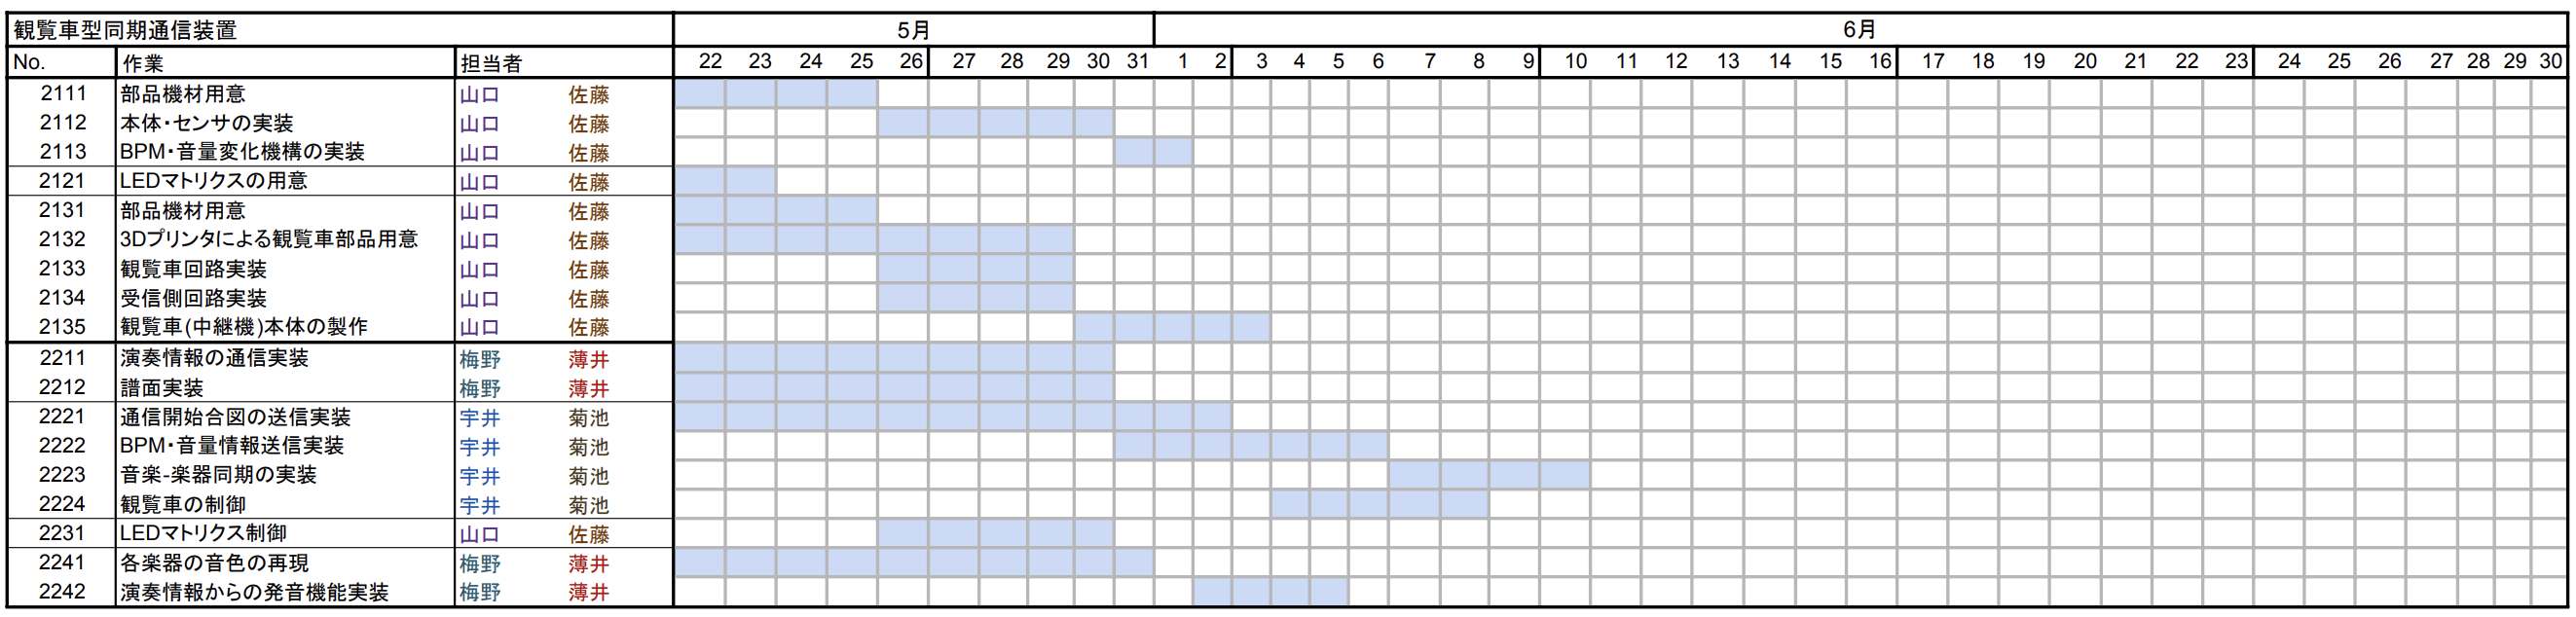
\includegraphics[width=0.8\columnwidth]{gant1.png} % 横幅を列幅の80%に指定
%    \caption{計画時のガントチャート} % 図の説明
%    \label{fig:gant1} % 本文中で参照するためのラベル
%\end{figure}

次に，現在のGCについて図\ref{fig:gant2}に示す．達成した項目は緑色で塗られている．

%\begin{figure}[htbp] % h:ここ, t:上, b:下, p:独立ページ
%    \centering % 中央揃え
%    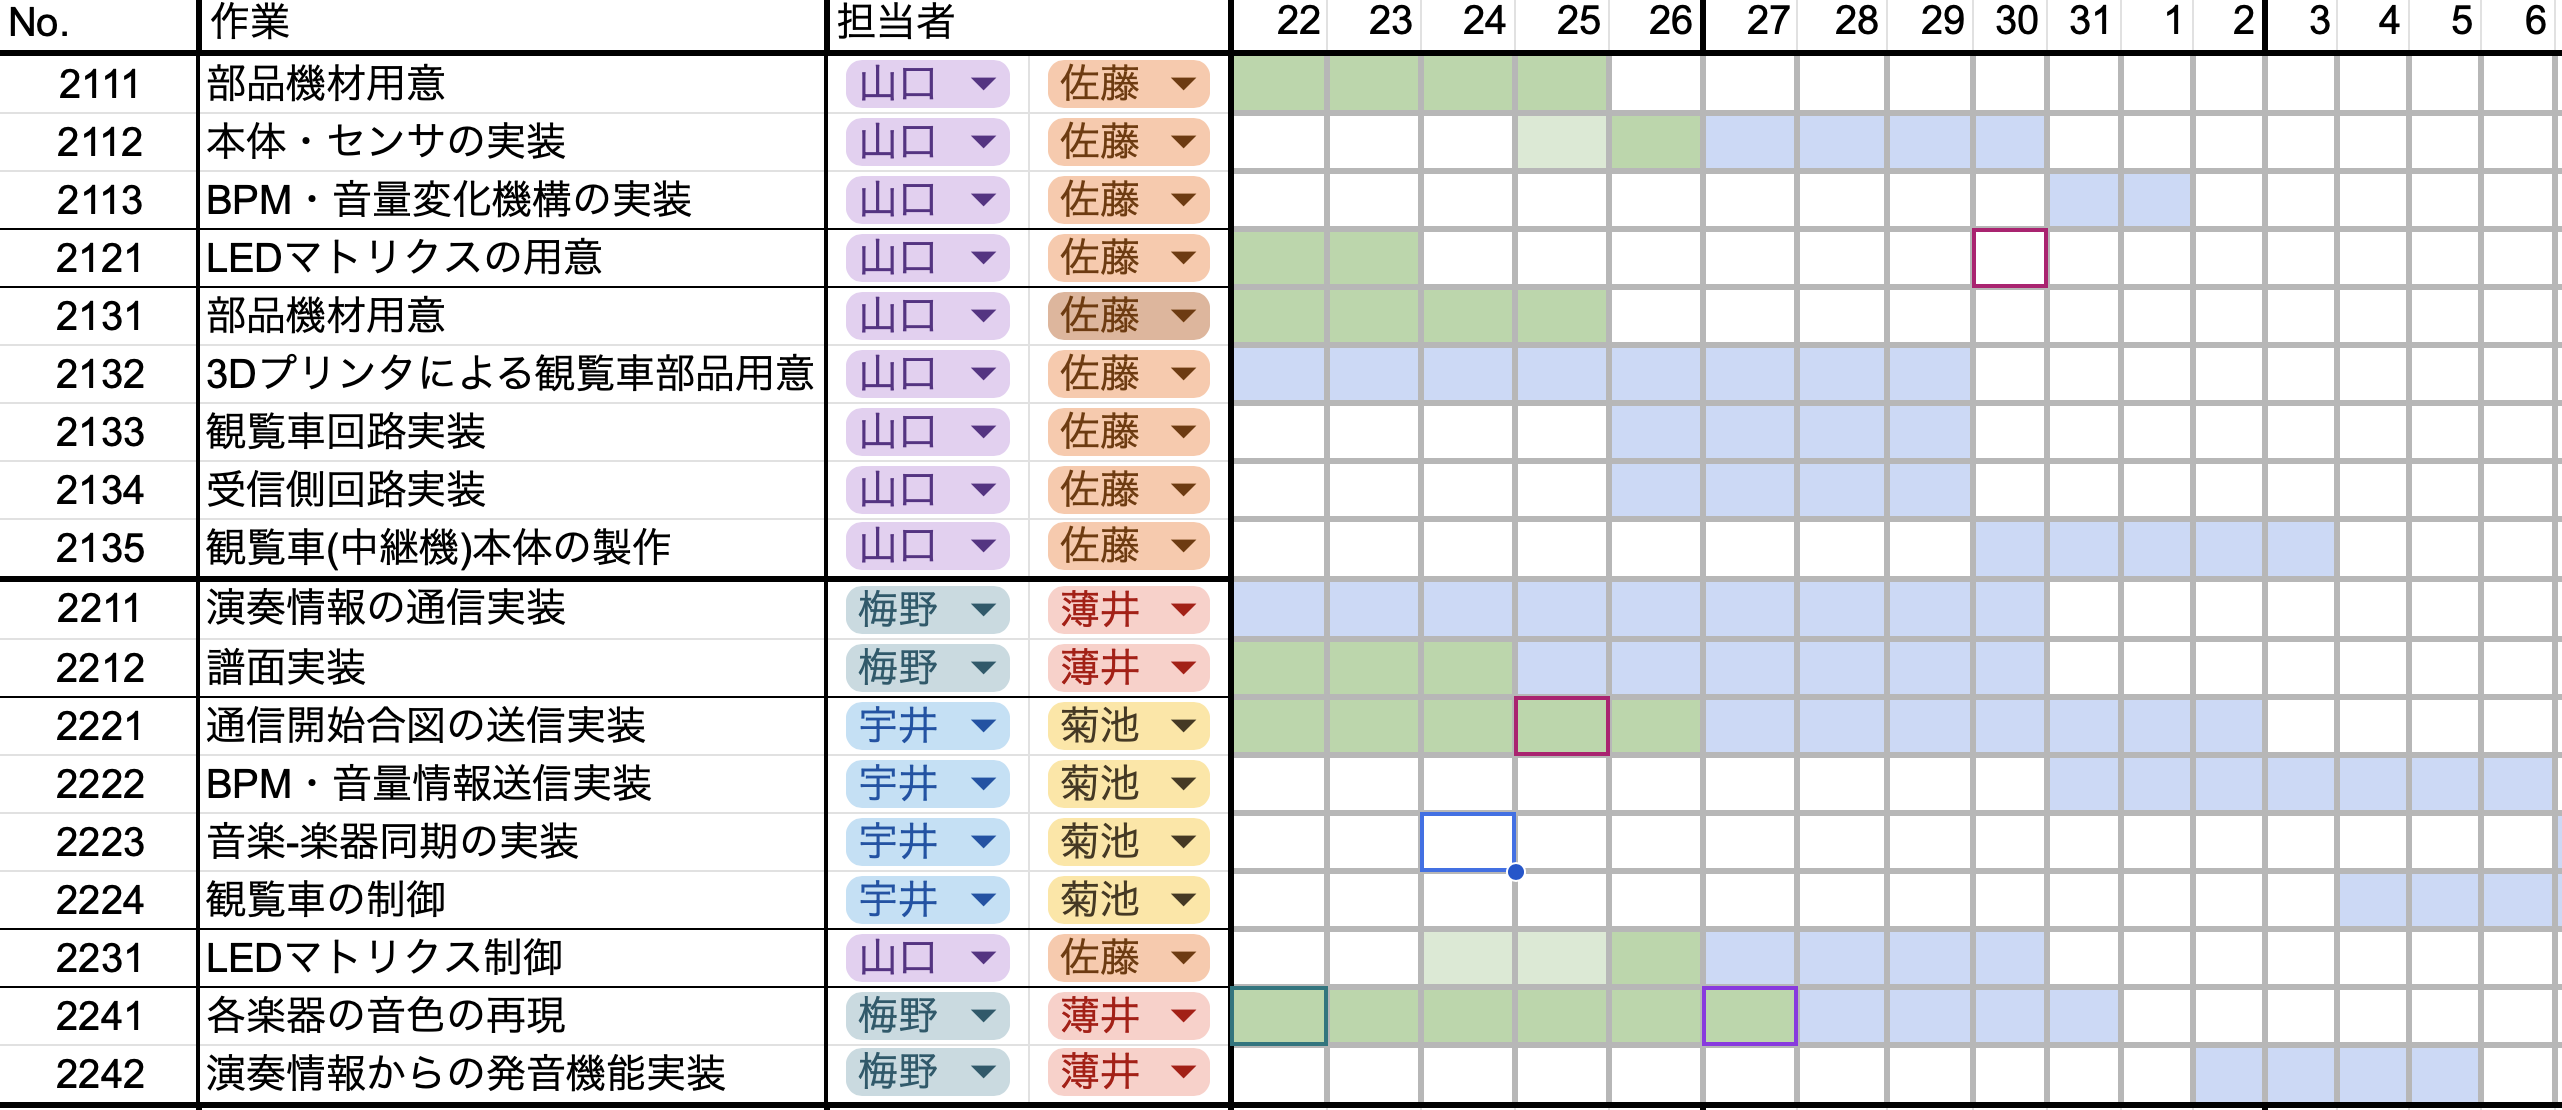
\includegraphics[width=0.8\columnwidth]{gant2.png} % 横幅を列幅の80%に指定
%    \caption{現在のガントチャート} % 図の説明
%    \label{fig:gant2} % 本文中で参照するためのラベル
%\end{figure}


\sectionrule


\section{課題管理}

\begin{tabularx}{\linewidth}{@{}p{3cm}Xllp{3.2cm}ll@{}}
\toprule
課題 & 発生原因 & 影響度 & 優先度 & 対策 & 期限 & 状態 \\
\midrule
可変抵抗器がブレッドボード上で安定接続できない（No.2112/2113に影響） & スライド式可変抵抗器の端子形状がブレッドボードに適合しないため． & 高 & 高 & スライド式を継続使用する場合は基盤にはんだ付けする．しぼり（回転式）の可変抵抗器に変更する場合は部品を貰う． & 6/9 & 対応中 \\
\midrule
LEDマトリクスが無表示になる & matrix操作が複数箇所に分散していたため． & 中 & 中 & 描画処理をDisplay.cppに集約し，表示を確定させた． & 5/30 & 対応済 \\
\bottomrule
\end{tabularx}

\medskip
※影響度＝プロジェクトへのインパクト

※優先度＝対応の緊急性

\sectionrule


\section{AI利用状況と検証（再現性重視）}

\subsection{利用内容}

\begin{itemize}
  \item 利用目的：設計・実装支援・レビュー

  \item 入力（プロンプト要旨）：
    \begin{itemize}
      \item 指揮デバイスのファームウェア作成にあたり，
      可変抵抗器の値をBPMの段階値へ写像する方法について質問した．

      \item LEDマトリクスが無表示になる不具合の原因と，
      その修正方法について質問した．
    \end{itemize}

  \item 出力概要：
    \begin{itemize}
      \item 可変抵抗器のアナログ値を段階値へ写像する実装方法の説明が得られた．

      \item LEDマトリクスの描画処理を一箇所に集約することで，
      表示を安定させる修正方針が得られた．
    \end{itemize}
\end{itemize}


\sectionrule

\subsection{検証方法}

\begin{itemize}

    \item 検証手法：
      \begin{itemize}
        \item AIが生成したファームウェアをArduino IDE上でコンパイル・実行し，
        可変抵抗器の操作に応じてBPM段階が正しく切り替わるかシリアルモニタで確認した．

        \item AIが提示した修正方針に従いLEDマトリクスの制御プログラムを修正し，
        実機で表示が安定するか確認した．

        \item AIの出力内容とArduino公式ドキュメントを比較し，
        使用関数や実装方法に誤りがないか確認した．
      \end{itemize}

      \item 参照資料：
      \begin{itemize}
        \item Arduino公式ドキュメント：
        \url{https://docs.arduino.cc/}

        \item Arduino Tutorials：
        \url{https://docs.arduino.cc/tutorials/}
      \end{itemize}

      \item 検証手順：
    \begin{enumerate}
      \item AIへ可変抵抗器の写像方法およびLEDマトリクスの不具合修正について質問した．

      \item AIが生成した内容をもとにファームウェアおよび制御プログラムを修正した．

      \item Arduinoへプログラムを書き込み，
      シリアルモニタおよび実機で動作を確認した．

      \item AIの出力内容をArduino公式ドキュメントと比較し，
      実装内容に誤りがないことを確認した．
    \end{enumerate}

\end{itemize}


\sectionrule

\subsection{ファクトチェック結果}


\begin{itemize}

    \item 一致点：
      \begin{itemize}
        \item AIが提示した可変抵抗器の読み取りおよび写像処理は，
        Arduino公式ドキュメントの内容と一致していた．

        \item LEDマトリクスの制御関数や描画処理についても，
        公式ドキュメントの記載と一致していた．
      \end{itemize}

      \item 不一致・疑義：
    \begin{itemize}
      \item 一部のサンプルコードにおいて，
      使用しているライブラリ名や関数名が実際の環境と異なる場合があり，
      修正が必要であった．
    \end{itemize}

  \item 最終判断：
    \begin{itemize}
      \item 一部採用
    \end{itemize}

    \item 根拠：
    \begin{itemize}
      \item Arduino公式ドキュメントとの比較により，
      AIの出力内容がおおむね正確であることを確認したため．

      \item 実際にファームウェアおよびLEDマトリクス制御を動作させ，
      正常に動作することを確認したため．
    \end{itemize}

\end{itemize}


\sectionrule


\section{次回計画}


\begin{itemize}

  \item 目標：指揮デバイスの完成，観覧車型中継機の製作着手
    \begin{itemize}
      \item 指揮デバイスのファームウェアを完成させ，
      本体・センサの実装を完了する．

      \item 観覧車型中継機の部品用意および本体製作に着手する．
    \end{itemize}

  \item 達成基準：
    \begin{itemize}
      \item 指揮デバイスが完成し，BPM・音量情報を送信できること．

      \item 観覧車型中継機の部品が用意され，製作に着手できていること．
    \end{itemize}

  \item 期限：
    \begin{itemize}
      \item 2026/6/9
    \end{itemize}

\end{itemize}


\sectionrule


\section{その他}

\begin{itemize}
  \item {}特になし．
\end{itemize}

\sectionrule


\section{付録}

\begin{itemize}
  \item 添付資料：
    \begin{itemize}
      \item No.3131のプログラム：\url{https://github.com/Sato907/3S_HCK1/tree/main/HCK1_group/HCK1_group_mywork/Display}
      \item No.2113のプログラム：\url{https://github.com/Sato907/3S_HCK1/tree/main/HCK1_group/HCK1_group_mywork/shiki_device}
      \item No.2134のプログラム：\url{https://github.com/Sato907/3S_HCK1/tree/main/HCK1_group/HCK1_group_mywork/cds_test}

    \end{itemize}

\end{itemize}

\sectionrule

\end{document}
